\begin{figure}[H]
    \centering
    \definecolor{strainblue}{RGB}{40,115,185}
    \definecolor{stressred}{RGB}{185,55,45}
    \definecolor{principalgray}{RGB}{125,130,135}
    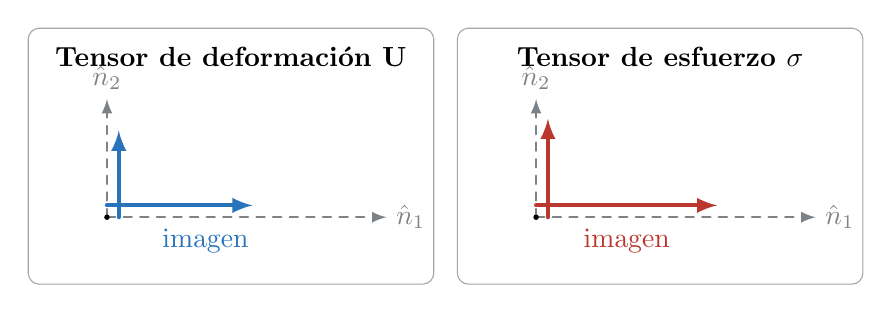
\begin{tikzpicture}[x=1cm,y=1cm,line cap=round,line join=round]
        % Paneles
        \draw[black!35,rounded corners=4pt] (0,0) rectangle (5.15,3.25);
        \draw[black!35,rounded corners=4pt] (5.45,0) rectangle (10.60,3.25);
        \node[font=\bfseries] at (2.575,2.88) {Tensor de deformación $\mathbf{U}$};
        \node[font=\bfseries] at (8.025,2.88) {Tensor de esfuerzo $\boldsymbol{\sigma}$};

        % Direcciones principales de deformación y sus imágenes bajo U
        \coordinate (OU) at (1.0,0.85);
        \draw[principalgray,dashed,-latex,line width=0.8pt] (OU) -- (4.55,0.85);
        \draw[principalgray,dashed,-latex,line width=0.8pt] (OU) -- (1.0,2.35);
        \draw[strainblue,-latex,line width=1.5pt] (1.0,1.00) -- (2.85,1.00);
        \draw[strainblue,-latex,line width=1.5pt] (1.15,0.85) -- (1.15,1.95);
        \node[principalgray,right] at (4.55,0.85) {$\hat{n}_1$};
        \node[principalgray,above] at (1.0,2.35) {$\hat{n}_2$};
        \node[strainblue,below] at (2.25,0.83) {imagen};
        \fill (OU) circle (0.035);

        % Las mismas direcciones principales y sus imágenes bajo sigma
        \coordinate (OS) at (6.45,0.85);
        \draw[principalgray,dashed,-latex,line width=0.8pt] (OS) -- (10.0,0.85);
        \draw[principalgray,dashed,-latex,line width=0.8pt] (OS) -- (6.45,2.35);
        \draw[stressred,-latex,line width=1.5pt] (6.45,1.00) -- (8.75,1.00);
        \draw[stressred,-latex,line width=1.5pt] (6.60,0.85) -- (6.60,2.10);
        \node[principalgray,right] at (10.0,0.85) {$\hat{n}_1$};
        \node[principalgray,above] at (6.45,2.35) {$\hat{n}_2$};
        \node[stressred,below] at (7.60,0.83) {imagen};
        \fill (OS) circle (0.035);
    \end{tikzpicture}
    \caption{Ambos tensores envían cada dirección principal a un vector paralelo a ella. Las longitudes de las flechas son esquemáticas y se muestran valores propios positivos; un valor propio negativo invertiría el sentido, pero no la dirección principal.}
\end{figure}